\documentclass[tikz,border=3pt]{standalone}
\usepackage[utf8]{inputenc}
\usepackage[T1]{fontenc}
\usepackage{lmodern}
\renewcommand{\familydefault}{\sfdefault}
\usepackage{sansmath}\sansmath
\usepackage{chemfig}
\usepackage{pgfplots}\pgfplotsset{compat=1.18,/pgf/number format/use comma,/pgf/number format/1000 sep={.}}
\usetikzlibrary{arrows.meta,calc,positioning,decorations.pathmorphing,patterns}
% paleta del sitio
\definecolor{nar}{HTML}{E8680C}\definecolor{narc}{HTML}{FFB35C}\definecolor{hielo}{HTML}{FFF3E8}
\definecolor{tinta}{HTML}{1D1D1F}\definecolor{gris}{HTML}{6E6E73}\definecolor{lila}{HTML}{7C5CF0}
\definecolor{azul}{HTML}{2F6FD6}\definecolor{menta}{HTML}{17A673}\definecolor{coral}{HTML}{E8342A}
\begin{document}
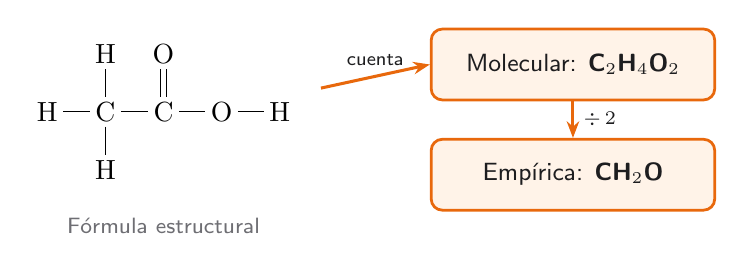
\begin{tikzpicture}
\node at (0,0) {\setchemfig{atom sep=2.1em}\chemfig{H-C(-[2]H)(-[6]H)-C(=[2]O)-O-H}};
\node[font=\sffamily\footnotesize,text=gris] at (0,-1.45) {Fórmula estructural};
\tikzset{caja/.style={draw=nar,fill=hielo,line width=1pt,rounded corners=4pt,minimum width=3.6cm,minimum height=0.9cm,align=center,font=\sffamily\small,text=tinta}}
\node[caja] (mo) at (5.2,0.6) {Molecular: \textbf{C$_2$H$_4$O$_2$}};
\node[caja] (em) at (5.2,-0.8) {Empírica: \textbf{CH$_2$O}};
\draw[-{Stealth[length=6pt]},line width=1.1pt,nar] (2.0,0.3) -- node[above,font=\sffamily\scriptsize,text=tinta] {cuenta} (mo.west);
\draw[-{Stealth[length=6pt]},line width=1.1pt,nar] (mo.south) -- node[right,font=\sffamily\scriptsize,text=tinta] {$\div\,2$} (em.north);
\end{tikzpicture}
\end{document}
